\documentclass{article}
\usepackage[spanish, es-tabla]{babel}
\usepackage[utf8]{inputenc}
\usepackage{graphicx}
\usepackage{subcaption}
\usepackage[colorlinks=true]{hyperref}
\title{Ejercicio 9}
\author{Daniel Rodríguez}
\date{\today}

\begin{document}
\maketitle
  La Figura \ref{fig:animales} muestra fotografías de varios animales.
  \begin{figure}[h!]
    \centering
    \begin{subfigure}[b]{0.4\textwidth}
      \centering
      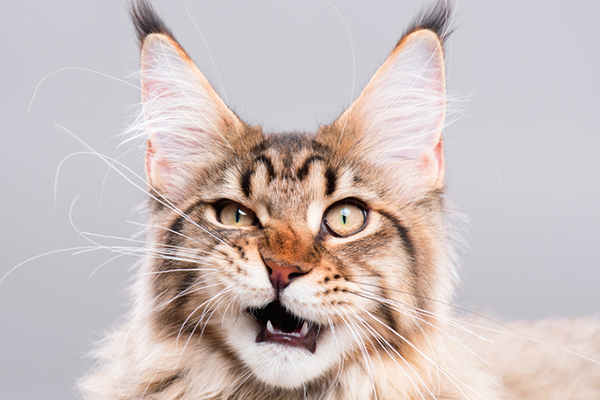
\includegraphics[height=0.5\linewidth]{../gato}
      \caption{Gato}
      \label{fig:gato}
    \end{subfigure}
    \begin{subfigure}[b]{0.4\textwidth}
      \centering
      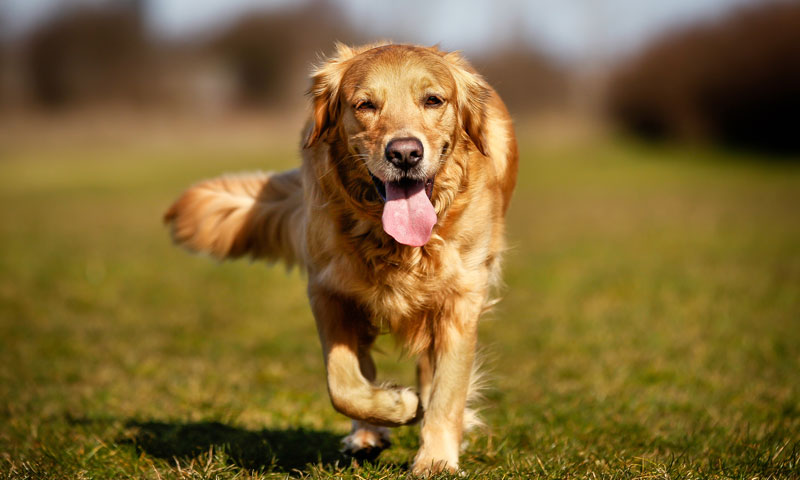
\includegraphics[height=0.5\linewidth]{../perro}
      \caption{Perro}
      \label{fig:perro}
    \end{subfigure} \\ [1ex]
    \begin{subfigure}[b]{0.4\textwidth}
      \centering
      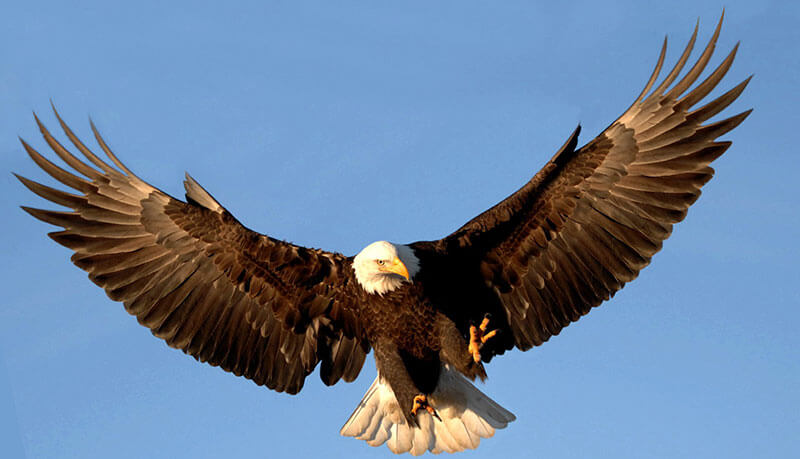
\includegraphics[height=0.5\linewidth]{../aguila}
      \caption{Águila}
      \label{fig:aguila}
    \end{subfigure} \\ [1ex]
    \begin{subfigure}[b]{0.3\textwidth}
      \centering
      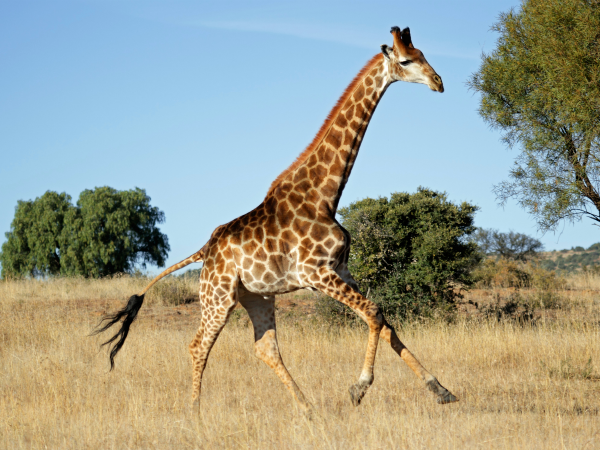
\includegraphics[height=0.5\linewidth]{../jirafa}
      \caption{Jirafa}
      \label{fig:jirafa}
    \end{subfigure}
    \begin{subfigure}[b]{0.3\textwidth}
      \centering
      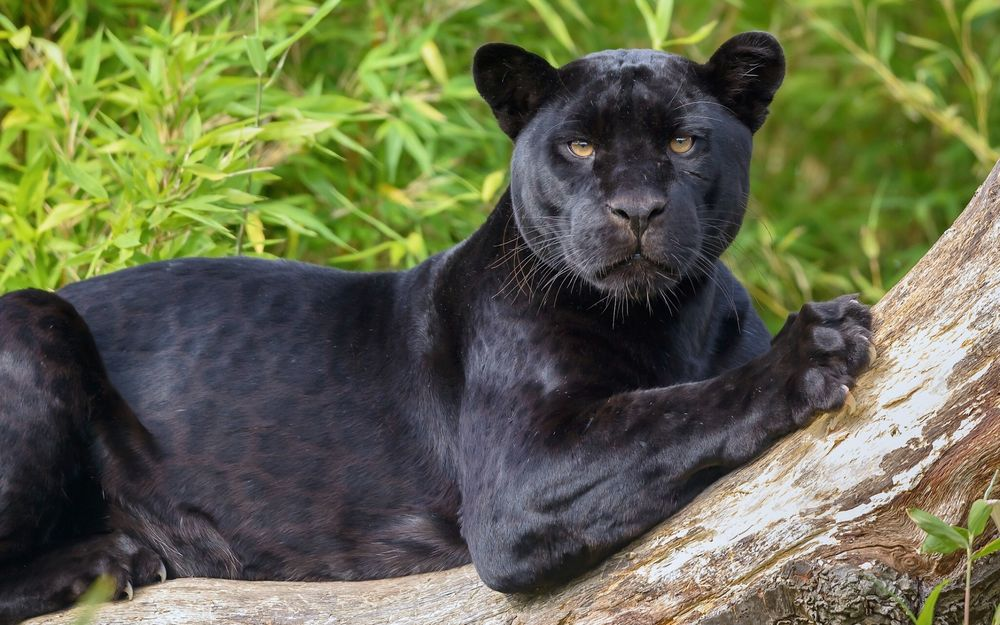
\includegraphics[height=0.5\linewidth]{../pantera}
      \caption{Pantera Negra}
      \label{fig:pantera}
    \end{subfigure}
    \begin{subfigure}[b]{0.3\textwidth}
      \centering
      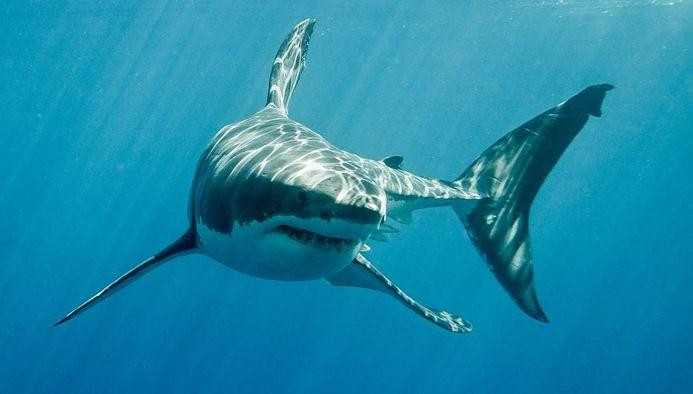
\includegraphics[height=0.5\linewidth]{../tiburon}
      \caption{Tiburón Blanco}
      \label{fig:tiburon}
    \end{subfigure}

  \caption{Varios tipos de animales}
  \label{fig:animales}
  \end{figure}
\end{document}
